\documentclass[8pt,aspectratio=169]{beamer}
\usepackage[utf8]{inputenc}
\usepackage{graphicx}
\usepackage{amsmath,amssymb}
\usepackage{algorithm2e}
\usepackage{listings}
\usepackage{xcolor}
\usepackage{tikz}
\usepackage{pgfplots}
\pgfplotsset{compat=1.17}
\usepackage{subfigure}
\usepackage{hyperref}
\usepackage{tcolorbox}
\usepackage{fontawesome5}

% Theme settings
\usetheme{Frankfurt}
\usecolortheme{seahorse}
\setbeamertemplate{navigation symbols}{}
\setbeamertemplate{footline}[frame number]
\setbeamertemplate{section in toc}[sections numbered]
\setbeamertemplate{subsection in toc}[subsections numbered]

% Custom colors
\definecolor{darkblue}{RGB}{0,51,102}
\definecolor{lightblue}{RGB}{173,216,230}
\definecolor{codegreen}{RGB}{0,128,0}
\definecolor{codegray}{RGB}{150,150,150}
\definecolor{codepurple}{RGB}{128,0,128}
\definecolor{backcolor}{RGB}{245,245,245}
\definecolor{prereqblue}{RGB}{230,240,255}
\definecolor{misconred}{RGB}{255,230,230}
\definecolor{checkgreen}{RGB}{230,255,230}
\definecolor{intuitionpurple}{RGB}{240,230,255}

% Code listing settings
\lstset{
    backgroundcolor=\color{backcolor},
    basicstyle=\ttfamily\tiny,
    breakatwhitespace=false,
    breaklines=true,
    captionpos=b,
    commentstyle=\color{codegreen},
    keywordstyle=\color{blue},
    numberstyle=\tiny\color{codegray},
    stringstyle=\color{codepurple},
    showstringspaces=false,
    frame=single,
    numbers=left,
    language=Python
}

% Include layout templates
% SLIDE LAYOUT TEMPLATES FOR NLP COURSE
% Three consistent layouts used throughout the course

% ==============================================================
% LAYOUT 1: CONCEPT SLIDE
% Used for: Theory, definitions, mathematical concepts
% Features: Title, main content area with bullets/equations, optional figure
% ==============================================================

\newcommand{\conceptslide}[3]{ % #1: title, #2: content, #3: optional figure
\begin{frame}[t]{#1}
    \begin{columns}[T]
        \begin{column}{0.6\textwidth}
            #2
        \end{column}
        \begin{column}{0.35\textwidth}
            \centering
            #3
        \end{column}
    \end{columns}
\end{frame}
}

% ==============================================================
% LAYOUT 2: CODE & IMPLEMENTATION SLIDE
% Used for: Code examples, algorithms, implementation details
% Features: Title, code block, explanation text
% ==============================================================

% Note: For code slides, use \begin{frame}[fragile] manually

\newcommand{\codeexplanation}[1]{%
    \vspace{0.5em}
    \small
    #1
}

\newcommand{\codeblock}[2][Python]{%
    \begin{lstlisting}[language=#1, basicstyle=\ttfamily\tiny]
#2
    \end{lstlisting}
}

\newcommand{\codeslide}[3]{%
    \begin{frame}[fragile]{#1}
    \begin{columns}[T]
        \column{0.55\textwidth}
        \codeblock{#2}
        \column{0.43\textwidth}
        \codeexplanation{#3}
    \end{columns}
    \end{frame}
}

% ==============================================================
% LAYOUT 3: RESULTS & VISUALIZATION SLIDE
% Used for: Experimental results, charts, comparisons
% Features: Title, large visualization area, key insights
% ==============================================================

\newcommand{\resultslide}[3]{ % #1: title, #2: visualization, #3: insights
\begin{frame}[t]{#1}
    \centering
    \vspace{-0.5em}
    #2
    \vspace{0.5em}
    
    \begin{block}{Key Insights}
        #3
    \end{block}
\end{frame}
}

% Additional utility commands for consistency

% Highlighted text
\newcommand{\highlight}[1]{\textcolor{blue}{\textbf{#1}}}

% Math notation shortcuts
\newcommand{\prob}[1]{P(#1)}
\newcommand{\given}{\mid}
\newcommand{\argmax}{\operatorname{argmax}}
\newcommand{\softmax}{\operatorname{softmax}}

% Standard figure size
\newcommand{\stdfigsizeinchins}{0.4\textwidth}

% For code blocks, use lstlisting directly:
% \begin{lstlisting}[language=Python]
% ... code ...
% \end{lstlisting}

% Equation highlight box
\newcommand{\eqbox}[1]{
    \begin{center}
    \colorbox{lightblue!20}{
        \parbox{0.8\textwidth}{
            \vspace{0.3em}
            \centering
            #1
            \vspace{0.3em}
        }
    }
    \end{center}
}

% Additional BSc-level commands
\newcommand{\prereq}[1]{\begin{tcolorbox}[colback=prereqblue,colframe=blue!50!black,title={\faIcon{book} Prerequisite}]#1\end{tcolorbox}}

\title[Week 4: Seq2Seq]{Natural Language Processing}
\subtitle{Week 4: Sequence-to-Sequence Models}
\institute{Breaking the Fixed-Length Barrier}
\author{}
\date{}

\begin{document}

% Title slide
\begin{frame}
    \titlepage
\end{frame}

% Learning Objectives with Prerequisites
\begin{frame}{Learning Objectives}
    \begin{columns}[T]
        \begin{column}{0.5\textwidth}
            \textbf{By the end of this lecture, you will:}
            \begin{enumerate}
                \item Understand why translation is hard for neural networks
                \item Design encoder-decoder architectures
                \item Identify the information bottleneck problem
                \item Master the attention mechanism
                \item Implement your own seq2seq model
            \end{enumerate}
        \end{column}
        \begin{column}{0.5\textwidth}
            \prereq{
                \textbf{Required Knowledge:}
                \begin{itemize}
                    \item RNNs and LSTMs (Week 3)
                    \item Backpropagation basics
                    \item Softmax function
                    \item Python/NumPy
                \end{itemize}
            }
            
            \vspace{0.5em}
            \textbf{Time Allocation:}
            \begin{itemize}
                \item Part 1: 15 min
                \item Part 2: 20 min
                \item Part 3: 15 min
                \item Part 4: 20 min
                \item Exercises: 20 min
            \end{itemize}
        \end{column}
    \end{columns}
\end{frame}

% Table of Contents
\begin{frame}{Week 4 Overview}
    \tableofcontents
\end{frame}

%=====================================
% PART 1: THE VARIABLE-LENGTH CHALLENGE
%=====================================

\section{Part 1: The Variable-Length Challenge}

% Start with intuition building
\begin{frame}[t]{Build Your Intuition: The Translation Problem}
    \textbf{Imagine you're translating a book from English to French. Would you:}
    \begin{itemize}
        \item A) Translate word-by-word in order?
        \item B) Read the whole sentence, understand it, then write in French?
        \item C) Look at chunks of 5 words at a time?
    \end{itemize}
    
    \textbf{Think:} Why doesn't option A work?
    
    \vspace{0.5em}
    \textbf{Example - Word-by-word translation fails:}
    \begin{itemize}
        \item English: ``I gave her the book yesterday''
        \item French: ``Je lui ai donné le livre hier''
        \item \textcolor{red}{Word-by-word back:} ``I her have given the book yesterday''
    \end{itemize}
    \textbf{The word order completely changes between languages!}
\end{frame}

\begin{frame}[fragile,t]{Why Can't We Just Use RNNs?}
    \begin{columns}[T]
        \begin{column}{0.6\textwidth}
            \textbf{Key Question:} \textit{You learned RNNs last week. Why can't we use them for translation?}
            
            \vspace{0.5em}
            \textbf{The Fundamental Problem:}
            \begin{itemize}
                \item RNNs expect: Input length = Output length
                \item Translation needs: Input length $\neq$ Output length
            \end{itemize}
            
            \vspace{0.5em}
            \textbf{Concrete Example:}
            \begin{itemize}
                \item EN: ``I love you'' (3 words)
                \item FR: ``Je t'aime'' (2 words)
                \item JP: ``Aishiteru'' (1 word)
                \item Which output position gets which input?
            \end{itemize}
        \end{column}
        \begin{column}{0.35\textwidth}
            \centering
            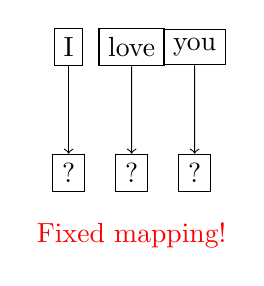
\begin{tikzpicture}[scale=0.8]
                % RNN expectation
                \node[draw] (in1) at (0,2) {I};
                \node[draw] (in2) at (1,2) {love};
                \node[draw] (in3) at (2,2) {you};
                
                \node[draw] (out1) at (0,0) {?};
                \node[draw] (out2) at (1,0) {?};
                \node[draw] (out3) at (2,0) {?};
                
                \draw[->] (in1) -- (out1);
                \draw[->] (in2) -- (out2);
                \draw[->] (in3) -- (out3);
                
                \node at (1,-1) {\textcolor{red}{Fixed mapping!}};
            \end{tikzpicture}
        \end{column}
    \end{columns}
\end{frame}

% Show real examples with numbers
\begin{frame}[t]{The Length Mismatch: Real Data}
    \textbf{Let's look at actual translation pairs:}
    
    \begin{center}
    \begin{tabular}{|l|l|c|c|}
        \hline
        \textbf{English} & \textbf{Target Language} & \textbf{EN Words} & \textbf{Target Words} \\
        \hline
        I love you & Je t'aime (French) & 3 & 2 \\
        I love you & Ich liebe dich (German) & 3 & 3 \\
        I love you & Aishiteru (Japanese) & 3 & 1 \\
        I love you & Wo ai ni (Chinese) & 3 & 3 \\
        I love you & Te amo (Spanish) & 3 & 2 \\
        \hline
        \multicolumn{4}{|c|}{\textit{Average length ratio: 3:2.2 (varies by 40\%!)}} \\
        \hline
    \end{tabular}
    \end{center}
    
    \vspace{0.5em}
    \begin{block}{Common Mistake: ``Just pad shorter sequences''}
        \begin{itemize}
            \item Where to pad? Beginning? End? Middle?
            \item Model doesn't know target length beforehand
            \item ``Je [PAD] t'aime'' $\neq$ ``Je t'aime [PAD]''
        \end{itemize}
    \end{block}
    
    
    \textbf{Question:} If padding doesn't work, what's the solution?
    \textit{Hint: How do human translators handle this?}
\end{frame}

% Historical evolution with timeline
\begin{frame}[t]{Evolution of Translation Approaches}
    \centering
    \vspace{-0.5em}
    \includegraphics[width=0.8\textwidth]{../figures/seq2seq_evolution_timeline.pdf}
    \vspace{0.5em}
    
    \begin{block}{Key Insights}
        \begin{itemize}
            \item \textbf{1950s-1990s}: Rule-based (dictionaries + grammar)
            \item \textbf{1990s-2014}: Statistical MT (phrase alignments)
            \item \textbf{2014}: \textbf{Seq2Seq breakthrough} - 15 BLEU improvement!
            \item \textbf{2017-now}: Transformers - Near human quality
        \end{itemize}
    \end{block}
\end{frame}

% The key insight
\begin{frame}[fragile,t]{The Brilliant Insight: Two-Stage Process}
    \textbf{Think about how YOU translate:}
    \begin{enumerate}
        \item \textbf{Read} and \textbf{understand} the entire sentence
        \item Form a mental \textbf{representation} of the meaning
        \item \textbf{Generate} the translation from that understanding
    \end{enumerate}
    
    \vspace{0.5em}
    \textbf{The Seq2Seq Solution (mimics human process):}
    
    \begin{center}
    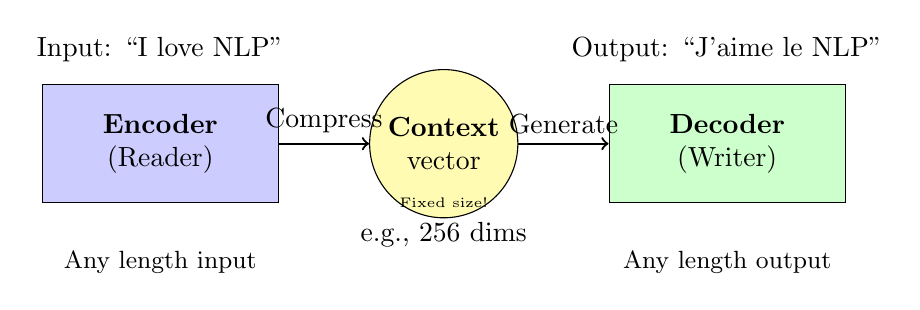
\begin{tikzpicture}[scale=0.9]
        % Stage 1: Encoding
        \node[draw, rectangle, minimum width=3cm, minimum height=1.5cm, fill=blue!20, align=center] (encoder) at (0,0) {\textbf{Encoder}\\(Reader)};
        \node[above of=encoder, node distance=1.2cm] {Input: ``I love NLP''};
        
        % Context vector
        \node[draw, circle, fill=yellow!30, align=center] (context) at (4,0) {\textbf{Context}\\vector};
        \node[below of=context, node distance=1cm, align=center] {\tiny Fixed size!\\e.g., 256 dims};
        
        % Stage 2: Decoding
        \node[draw, rectangle, minimum width=3cm, minimum height=1.5cm, fill=green!20, align=center] (decoder) at (8,0) {\textbf{Decoder}\\(Writer)};
        \node[above of=decoder, node distance=1.2cm] {Output: ``J'aime le NLP''};
        
        % Arrows with labels
        \draw[->, thick] (encoder) -- (context) node[midway, above] {Compress};
        \draw[->, thick] (context) -- (decoder) node[midway, above] {Generate};
        
        % Annotations
        \node[below of=encoder, node distance=1.5cm] {\small Any length input};
        \node[below of=decoder, node distance=1.5cm] {\small Any length output};
    \end{tikzpicture}
    \end{center}
    
    
    \textbf{Key Question:} Why do we need TWO networks instead of modifying one RNN?
\end{frame}

%=====================================
% PART 2: THE ENCODER-DECODER ARCHITECTURE  
%=====================================

\section{Part 2: The Encoder-Decoder Architecture}

% Build intuition first
\begin{frame}[fragile,t]{Building Intuition: The Encoder}
    \textbf{The encoder is like a reader that builds understanding:}
    \begin{itemize}
        \item Reads words one by one (like you reading this)
        \item Updates its understanding with each word
        \item Final understanding = complete meaning
    \end{itemize}
    
    \textbf{Step-by-step encoding of ``The cat sat'':}
    
    \begin{center}
    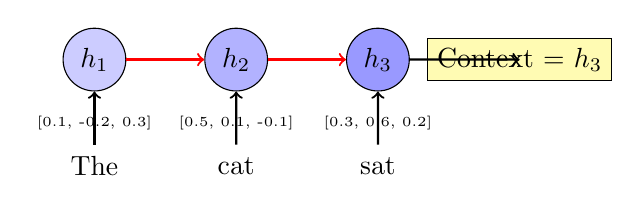
\begin{tikzpicture}[scale=0.9]
        % Words and hidden states
        \node at (0, 0) {The};
        \node at (2, 0) {cat};
        \node at (4, 0) {sat};
        
        % Hidden states with values
        \node[draw, circle, fill=blue!20] (h1) at (0, 1.5) {$h_1$};
        \node[draw, circle, fill=blue!30] (h2) at (2, 1.5) {$h_2$};
        \node[draw, circle, fill=blue!40] (h3) at (4, 1.5) {$h_3$};
        
        % Connections
        \draw[->, thick] (0, 0.3) -- (h1);
        \draw[->, thick] (2, 0.3) -- (h2);
        \draw[->, thick] (4, 0.3) -- (h3);
        
        \draw[->, thick, red] (h1) -- (h2);
        \draw[->, thick, red] (h2) -- (h3);
        
        % Actual values
        \node[below of=h1, node distance=0.8cm] {\tiny [0.1, -0.2, 0.3]};
        \node[below of=h2, node distance=0.8cm] {\tiny [0.5, 0.1, -0.1]};
        \node[below of=h3, node distance=0.8cm] {\tiny [0.3, 0.6, 0.2]};
        
        % Context
        \node[draw, rectangle, fill=yellow!30] at (6, 1.5) {Context = $h_3$};
        \draw[->, thick] (h3) -- (6, 1.5);
    \end{tikzpicture}
    \end{center}
    
    \textbf{Example - Track how the hidden state changes:}
    \begin{itemize}
        \item ``The'' $\rightarrow$ General/article context
        \item ``The cat'' $\rightarrow$ Animal/subject identified  
        \item ``The cat sat'' $\rightarrow$ Complete action understood
    \end{itemize}
\end{frame}

% Mathematical formulation with explanations
\begin{frame}[fragile,t]{Encoder Mathematics (With Intuition)}
    \begin{columns}[T]
        \begin{column}{0.6\textwidth}
    \textbf{What happens at each step:}
    
    \eqbox{
        \textbf{For each input word $x_t$ at time $t$:}\\
        \vspace{0.3em}
        $h_t^{enc} = \text{LSTM}(x_t, h_{t-1}^{enc})$\\
        \vspace{0.3em}
        Breaking this down:
        \begin{itemize}
            \item $x_t$ = current word (embedded as vector)
            \item $h_{t-1}^{enc}$ = what we understood so far
            \item $h_t^{enc}$ = updated understanding
        \end{itemize}
    }
    
    \vspace{0.5em}
    \textbf{Concrete dimensions:}
    \begin{itemize}
        \item Word embedding: $x_t \in \mathbb{R}^{100}$ 
        \item Hidden state: $h_t \in \mathbb{R}^{256}$
        \item Context: $c = h_T^{enc} \in \mathbb{R}^{256}$
    \end{itemize}
    
    \textbf{Quick note:} Processing 10 words $\rightarrow$ 10 hidden states (one per word)
        \end{column}
        \begin{column}{0.35\textwidth}
            \centering
    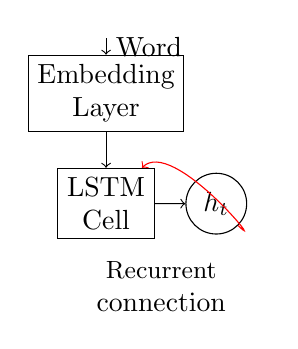
\begin{tikzpicture}[scale=0.7]
        % Visual representation
        \node[draw, rectangle, align=center] (embed) at (0,0) {Embedding\\Layer};
        \node[draw, rectangle, align=center] (lstm) at (0,-2) {LSTM\\Cell};
        \node[draw, circle] (hidden) at (2,-2) {$h_t$};
        
        \draw[->] (0,1) -- (embed) node[midway, right] {Word};
        \draw[->] (embed) -- (lstm);
        \draw[->] (lstm) -- (hidden);
        \draw[->, red] (hidden) to[out=-45,in=45] (lstm);
        
        \node[align=center] at (1,-3.5) {\small Recurrent\\connection};
    \end{tikzpicture}
        \end{column}
    \end{columns}
\end{frame}

% Implementation
\begin{frame}[fragile,t]{Encoder Implementation (Simplified)}
    \textbf{Let's implement what we just learned} - it's simpler than you think!
    
    \begin{columns}[T]
        \column{0.55\textwidth}
        \begin{lstlisting}[language=Python]
class Encoder:
    def __init__(self, vocab_size, hidden_dim):
        # Two components only!
        self.embedding = Embedding(vocab_size, 100)
        self.lstm = LSTM(100, hidden_dim)
        
    def forward(self, sentence):
        # sentence = ["I", "love", "NLP"]
        
        # Start with zero understanding
        hidden = zeros(hidden_dim)  # [0,0,...,0]
        
        # Process each word
        for word in sentence:
            # Convert word to vector
            embed = self.embedding[word]  # 100d
            
            # Update our understanding
            hidden = self.lstm(embed, hidden)  # 256d
            
        # Final understanding
        context = hidden
        return context  # This is all decoder gets!
        \end{lstlisting}
        
        \column{0.43\textwidth}
        \textbf{Line-by-line walkthrough:}
        
        \small
        \begin{itemize}
            \item \textbf{Lines 3-4}: Just 2 components!
            \item \textbf{Line 10}: Start knowing nothing
            \item \textbf{Lines 13-17}: Core loop
            \begin{itemize}
                \small
                \item Get word vector
                \item Update understanding
                \item Keep only latest
            \end{itemize}
            \item \textbf{Line 20}: Final state = context
        \end{itemize}
        
        \vspace{0.5em}
        \begin{block}{Key Insight}
            Context size is \textbf{always the same}:
            \begin{itemize}
                \item 3 words $\rightarrow$ 256 dims
                \item 100 words $\rightarrow$ Still 256 dims!
            \end{itemize}
            \textit{This fixed size is both a strength and weakness...}
        \end{block}
    \end{columns}
\end{frame}

% Decoder intuition
\begin{frame}[fragile,t]{Building Intuition: The Decoder}
    \textbf{The decoder is like a writer that generates from understanding:}
    \begin{itemize}
        \item Starts with the context (understanding)
        \item Generates one word at a time
        \item Each word depends on context + previous words
    \end{itemize}
    
    \textbf{Generation process for ``Le chat'':}
    
    \begin{center}
    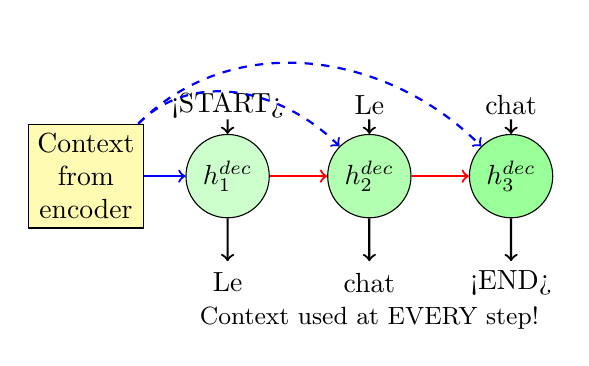
\begin{tikzpicture}[scale=0.9]
        % Context
        \node[draw, rectangle, fill=yellow!30, align=center] (context) at (-1, 1.5) {Context\\from\\encoder};
        
        % Generation steps
        \node[draw, circle, fill=green!20] (h1) at (1, 1.5) {$h_1^{dec}$};
        \node[draw, circle, fill=green!30] (h2) at (3, 1.5) {$h_2^{dec}$};
        \node[draw, circle, fill=green!40] (h3) at (5, 1.5) {$h_3^{dec}$};
        
        % Generated words
        \node at (1, 0) {Le};
        \node at (3, 0) {chat};
        \node at (5, 0) {<END>};
        
        % Previous words fed back
        \node at (1, 2.5) {<START>};
        \node at (3, 2.5) {Le};
        \node at (5, 2.5) {chat};
        
        % Connections
        \draw[->, thick, blue] (context) -- (h1);
        \draw[->, thick, blue, dashed] (context) to[out=45,in=135] (h2);
        \draw[->, thick, blue, dashed] (context) to[out=45,in=135] (h3);
        
        \draw[->, thick] (1, 2.3) -- (h1);
        \draw[->, thick] (3, 2.3) -- (h2);
        \draw[->, thick] (5, 2.3) -- (h3);
        
        \draw[->, thick] (h1) -- (1, 0.3);
        \draw[->, thick] (h2) -- (3, 0.3);
        \draw[->, thick] (h3) -- (5, 0.3);
        
        \draw[->, thick, red] (h1) -- (h2);
        \draw[->, thick, red] (h2) -- (h3);
        
        \node at (3, -0.5) {\small Context used at EVERY step!};
    \end{tikzpicture}
    \end{center}
\end{frame}

% Decoder mathematics
\begin{frame}[t]{Decoder Mathematics (With Intuition)}
    \begin{columns}[T]
        \begin{column}{0.6\textwidth}
    \textbf{Generation at each step:}
    
    \eqbox{
        \textbf{For each output position $t$:}\\
        \vspace{0.3em}
        $h_t^{dec} = \text{LSTM}(y_{t-1}, h_{t-1}^{dec}, c)$\\
        $P(y_t | y_{<t}, c) = \softmax(W \cdot h_t^{dec} + b)$\\
        \vspace{0.3em}
        Breaking this down:
        \begin{itemize}
            \item $y_{t-1}$ = previous word we generated
            \item $c$ = context from encoder (always same!)
            \item $h_t^{dec}$ = decoder's current state
            \item $P(y_t|...)$ = probability of each word
        \end{itemize}
    }
    
    \vspace{0.5em}
    \textbf{Concrete example:}
    \begin{itemize}
        \item Generating ``chat'' after ``Le''
        \item Previous: $y_{t-1}$ = ``Le'' $\rightarrow$ [0.2, 0.1, ...]
        \item Context: $c$ = [0.3, 0.6, 0.2, ...] (256d)
        \item Output: P(``chat'') = 0.7, P(``chien'') = 0.2, ...
    \end{itemize}
        \end{column}
        \begin{column}{0.35\textwidth}
            \centering
    \includegraphics[width=\textwidth]{../figures/encoder_decoder_flow.pdf}
        \end{column}
    \end{columns}
\end{frame}

% Teacher forcing
\begin{frame}[t]{Training Trick: Teacher Forcing}
    \textbf{Problem:} How do we train when the model makes mistakes early on?
    
    \begin{columns}[T]
        \column{0.5\textwidth}
        \textbf{During Training (Teacher Forcing):}
        \begin{itemize}
            \item Feed the TRUE previous word
            \item Not the model's prediction
            \item Speeds up training dramatically
        \end{itemize}
        
        \vspace{0.5em}
        Example: Teaching ``Le chat noir''
        \begin{enumerate}
            \item Input: <START> $\rightarrow$ Predict: ``Le''
            \item Input: ``Le'' (true) $\rightarrow$ Predict: ``chat''
            \item Input: ``chat'' (true) $\rightarrow$ Predict: ``noir''
        \end{enumerate}
        
        \column{0.5\textwidth}
        \textbf{During Testing (No Teacher):}
        \begin{itemize}
            \item Feed MODEL's previous prediction
            \item No true words available!
            \item Errors can accumulate
        \end{itemize}
        
        \vspace{0.5em}
        Example: Generating translation
        \begin{enumerate}
            \item Input: <START> $\rightarrow$ Generates: ``Le''
            \item Input: ``Le'' (generated) $\rightarrow$ Generates: ``chat''
            \item Input: ``chat'' (generated) $\rightarrow$ Generates: ``noir''
        \end{enumerate}
    \end{columns}
    
    \vspace{0.5em}
    \begin{block}{Important Distinction}
        \textcolor{red}{\textbf{Common mistake:}} ``Teacher forcing at test time''\\
        Remember: During testing, you don't have the correct translation to feed back!
    \end{block}
\end{frame}

%=====================================
% PART 3: THE INFORMATION BOTTLENECK PROBLEM
%=====================================

\section{Part 3: The Information Bottleneck Problem}

% Intuition first
\begin{frame}[fragile,t]{The Compression Problem}
    \textbf{Imagine compressing a book into a single paragraph:}
    \begin{itemize}
        \item Short story (5 pages) $\rightarrow$ Paragraph: Works well!
        \item Novel (300 pages) $\rightarrow$ Paragraph: Loses details
        \item Encyclopedia $\rightarrow$ Paragraph: Impossible!
    \end{itemize}
    
    \textit{Same problem with seq2seq: Longer input $\rightarrow$ More information loss}
    
    \textbf{The Bottleneck Visualization:}
    
    \begin{center}
    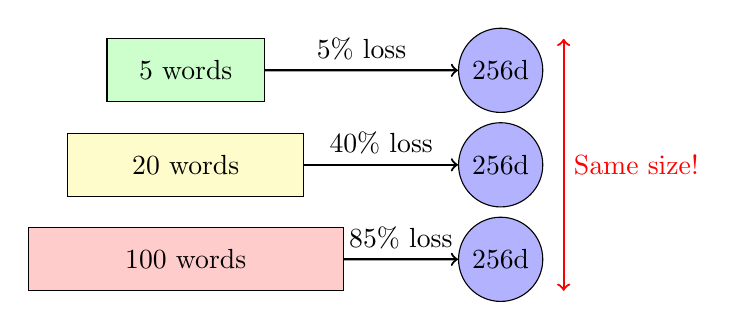
\begin{tikzpicture}[scale=0.8]
        % Different length inputs
        \node[draw, rectangle, minimum width=2cm, minimum height=0.8cm, fill=green!20] (short) at (0, 2) {5 words};
        \node[draw, rectangle, minimum width=3cm, minimum height=0.8cm, fill=yellow!20] (medium) at (0, 0.5) {20 words};
        \node[draw, rectangle, minimum width=4cm, minimum height=0.8cm, fill=red!20] (long) at (0, -1) {100 words};
        
        % Same size context
        \node[draw, circle, fill=blue!30] (context1) at (5, 2) {256d};
        \node[draw, circle, fill=blue!30] (context2) at (5, 0.5) {256d};
        \node[draw, circle, fill=blue!30] (context3) at (5, -1) {256d};
        
        % Arrows with loss indicators
        \draw[->, thick] (short) -- (context1) node[midway, above] {5\% loss};
        \draw[->, thick] (medium) -- (context2) node[midway, above] {40\% loss};
        \draw[->, thick] (long) -- (context3) node[midway, above] {85\% loss};
        
        % Same size indicator
        \draw[<->, thick, red] (6, 2.5) -- (6, -1.5) node[midway, right] {Same size!};
    \end{tikzpicture}
    \end{center}
    
    
    \textbf{Question:} Why can't we just use a bigger context vector?
\end{frame}

% Show with real numbers
\begin{frame}[t]{Information Theory Analysis}
    \centering
    \vspace{-0.5em}
    \includegraphics[width=0.7\textwidth]{../figures/bottleneck_visualization.pdf}
    \vspace{0.5em}
    
    \begin{block}{Key Insights}
        \textbf{The bottleneck effect:}
        \begin{itemize}
            \item Short sentences (5 words) $\rightarrow$ Easy to compress
            \item Medium sentences (20 words) $\rightarrow$ Some loss but manageable
            \item Long sentences (100 words) $\rightarrow$ Major information loss
            \item \textbf{Rule of thumb:} Performance drops significantly after 30 words
        \end{itemize}
    \end{block}
\end{frame}

% Experimental evidence
\begin{frame}[t]{Where Information Gets Lost}
    \textbf{Let's trace what happens to a long sentence:}
    
    \small
    \textit{``The International Conference on Machine Learning, which is one of the premier venues for presenting research in machine learning and attracts submissions from researchers around the world, accepted our paper.''}
    
    \vspace{0.5em}
    \textbf{What the context vector captures:}
    \begin{columns}[T]
        \column{0.5\textwidth}
        \textcolor{green}{\textbf{Y Preserved:}}
        \begin{itemize}
            \item General topic (ML conference)
            \item Sentiment (positive - accepted)
            \item Basic structure (statement)
        \end{itemize}
        
        \column{0.5\textwidth}
        \textcolor{red}{\textbf{X Lost:}}
        \begin{itemize}
            \item ``International'' detail
            \item ``premier venues'' specificity
            \item ``researchers around the world''
            \item Exact conference name
        \end{itemize}
    \end{columns}
    
    \vspace{0.5em}
    \textbf{Experimental Results (Bahdanau et al., 2015):}
    \begin{center}
    \begin{tabular}{|l|c|c|}
        \hline
        \textbf{Sentence Length} & \textbf{BLEU Score} & \textbf{Quality} \\
        \hline
        < 10 words & 35.2 & Excellent \\
        10-20 words & 28.5 & Good \\
        20-30 words & 19.3 & Mediocre \\
        > 30 words & 9.7 & Poor \\
        \hline
    \end{tabular}
    \end{center}
    
    \textbf{Performance drops 72\% for long sentences!}
\end{frame}

%=====================================
% PART 4: ATTENTION MECHANISM - THE GAME CHANGER
%=====================================

\section{Part 4: Attention Mechanism - The Game Changer}

% Human intuition
\begin{frame}[t]{How Humans Translate (The Key Insight)}
    \textbf{When you translate ``The black cat sat on the mat'' to French:}
    \begin{itemize}
        \item For ``Le'' $\rightarrow$ You look at ``The''
        \item For ``chat'' $\rightarrow$ You look at ``cat''
        \item For ``noir'' $\rightarrow$ You look at ``black''
        \item You DON'T look at all words equally!
    \end{itemize}
    
    \textbf{Let's track what we look at:}
    
    \begin{center}
    \begin{tabular}{|l|l|l|}
        \hline
        \textbf{Generating} & \textbf{Looking at} & \textbf{Attention Weight} \\
        \hline
        ``Le'' & Mainly ``The'' & 0.8 on ``The'', 0.2 others \\
        ``chat'' & Mainly ``cat'' & 0.7 on ``cat'', 0.3 others \\
        ``noir'' & Mainly ``black'' & 0.6 on ``black'', 0.4 others \\
        ``s'est assis'' & Mainly ``sat'' & 0.9 on ``sat'', 0.1 others \\
        ``sur'' & Mainly ``on'' & 0.8 on ``on'', 0.2 others \\
        ``le'' & Mainly ``the'' & 0.7 on ``the'', 0.3 others \\
        ``tapis'' & Mainly ``mat'' & 0.85 on ``mat'', 0.15 others \\
        \hline
    \end{tabular}
    \end{center}
    
    
    \textbf{Key Insight:} What if the decoder could do this too - look back at specific encoder states?
\end{frame}

% The attention solution
\begin{frame}[t]{The Attention Solution}
    \begin{columns}[T]
        \begin{column}{0.6\textwidth}
    \textbf{Instead of one context vector:}
    \begin{itemize}
        \item Keep ALL encoder hidden states
        \item Let decoder choose what to look at
        \item Different focus for each output word
    \end{itemize}
    
    \vspace{0.5em}
    \textbf{The 3-step attention process:}
    
    \eqbox{
        1. \textbf{Score:} How relevant is each encoder state?\\
        $e_{ti} = \text{score}(h_t^{dec}, h_i^{enc})$
        
        2. \textbf{Normalize:} Convert to probabilities\\
        $\alpha_{ti} = \frac{\exp(e_{ti})}{\sum_j \exp(e_{tj})}$
        
        3. \textbf{Combine:} Weighted sum\\
        $c_t = \sum_i \alpha_{ti} \cdot h_i^{enc}$
    }
    
    \textbf{Example:} For ``chat'', attention weights = [0.1, 0.7, 0.2]
    \begin{itemize}
        \item 10\% focus on ``The''
        \item \textbf{70\% focus on ``cat''} $\leftarrow$ Makes sense!
        \item 20\% focus on ``sat''
    \end{itemize}
        \end{column}
        \begin{column}{0.35\textwidth}
            \centering
    \includegraphics[width=\textwidth]{../figures/attention_heatmap.pdf}
        \end{column}
    \end{columns}
\end{frame}

% Concrete calculation
\begin{frame}[t]{Attention Calculation: Step by Step}
    \textbf{Let's calculate attention for generating ``chat'':}
    
    \begin{columns}[T]
        \column{0.6\textwidth}
        \textbf{Step 1: Score each source word}
        
        Current decoder state: $h_2^{dec} = [0.5, -0.2, 0.8]$
        
        \small
        \begin{tabular}{|l|l|c|}
            \hline
            \textbf{Word} & \textbf{Hidden State} & \textbf{Score} \\
            \hline
            ``The'' & [0.1, 0.2, 0.1] & 0.09 \\
            ``cat'' & [0.8, 0.1, 0.7] & 0.94 \\
            ``sat'' & [0.2, 0.3, 0.2] & 0.20 \\
            \hline
        \end{tabular}
        
        \vspace{0.5em}
        \textbf{Step 2: Apply softmax}
        \begin{align*}
            \alpha_1 &= \frac{e^{0.09}}{e^{0.09} + e^{0.94} + e^{0.20}} = 0.27\\
            \alpha_2 &= \frac{e^{0.94}}{...} = \textcolor{red}{0.63}\\
            \alpha_3 &= \frac{e^{0.20}}{...} = 0.10
        \end{align*}
        
        \column{0.35\textwidth}
        \textbf{Step 3: Weighted combination}
        
        \small
        $c_2 = 0.27 \cdot h_1^{enc} +$\\
        $\phantom{c_2 = }0.63 \cdot h_2^{enc} +$\\
        $\phantom{c_2 = }0.10 \cdot h_3^{enc}$
        
        \vspace{0.5em}
        \textbf{Result:}
        \begin{itemize}
            \item 63\% attention on ``cat''
            \item Correct word alignment!
            \item Context is mostly ``cat''
        \end{itemize}
        
        \vspace{0.5em}
        \includegraphics[width=\textwidth]{../figures/attention_visualization.pdf}
    \end{columns}
\end{frame}

% Implementation
\begin{frame}[fragile,t]{Attention Implementation}
    \begin{columns}[T]
        \column{0.55\textwidth}
        \begin{lstlisting}[language=Python]
def attention(decoder_hidden, encoder_outputs):
    """
    decoder_hidden: current state [256]
    encoder_outputs: all states [seq_len, 256]
    """
    scores = []
    
    # Step 1: Score each encoder output
    for enc_out in encoder_outputs:
        # Dot product similarity
        score = dot(decoder_hidden, enc_out)
        scores.append(score)
    
    # Step 2: Normalize with softmax
    scores = array(scores)
    exp_scores = exp(scores - max(scores))
    weights = exp_scores / sum(exp_scores)
    
    # Step 3: Weighted combination
    context = zeros_like(decoder_hidden)
    for i, enc_out in enumerate(encoder_outputs):
        context += weights[i] * enc_out
    
    return context, weights

# Usage in decoder:
for t in range(max_length):
    context, attn = attention(hidden, all_enc)
    # Use context instead of fixed vector!
        \end{lstlisting}
        
        \column{0.43\textwidth}
        \textbf{Key improvements:}
        
        \begin{itemize}
            \item \textbf{Line 9-11}: Score relevance
            \item \textbf{Line 15-16}: Softmax for probabilities
            \item \textbf{Line 19-21}: Custom context
        \end{itemize}
        
        \vspace{0.5em}
        \textbf{Example with 10 source words:}
        \begin{itemize}
            \item 10 attention weights
            \item Sum to 1.0
            \item Different for each output!
        \end{itemize}
        
        \vspace{0.5em}
        \textbf{Important Note:}
        \begin{itemize}
            \item \textbf{Q:} ``Does attention look at future words?''
            \item \textbf{A:} No! Only at encoder (source) states, never future target words.
        \end{itemize}
    \end{columns}
\end{frame}

% Different attention types
\begin{frame}[t]{Types of Attention Mechanisms}
    \textbf{Three ways to compute attention scores:}
    
    \begin{columns}[T]
        \column{0.5\textwidth}
        \textbf{1. Dot Product (Luong)}
        \eqbox{
            $e_{ti} = h_t^{dec} \cdot h_i^{enc}$
        }
        \begin{itemize}
            \item Simplest and fastest
            \item No parameters to learn
            \item Works well in practice
        \end{itemize}
        
        \vspace{0.5em}
        \textbf{2. Scaled Dot Product}
        \eqbox{
            $e_{ti} = \frac{h_t^{dec} \cdot h_i^{enc}}{\sqrt{d}}$
        }
        \begin{itemize}
            \item Used in Transformers
            \item Prevents large values
            \item More stable gradients
        \end{itemize}
        
        \column{0.5\textwidth}
        \textbf{3. Additive (Bahdanau)}
        \eqbox{
            $e_{ti} = v^T \tanh(W_1 h_t^{dec} + W_2 h_i^{enc})$
        }
        \begin{itemize}
            \item Original attention paper
            \item More parameters
            \item More flexible
        \end{itemize}
        
        \vspace{0.5em}
        \textbf{Performance comparison:}
        \begin{center}
        \small
        \begin{tabular}{|l|c|c|}
            \hline
            \textbf{Type} & \textbf{BLEU} & \textbf{Speed} \\
            \hline
            Dot Product & 31.2 & Fast \\
            Scaled & 31.5 & Fast \\
            Additive & 31.7 & Slower \\
            \hline
        \end{tabular}
        \end{center}
    \end{columns}
\end{frame}

% Results with attention - NEW visualization
\begin{frame}[t]{The Impact of Attention: Step-by-Step}
    \centering
    \vspace{-1em}
    \includegraphics[width=0.95\textwidth]{../figures/attention_flow_steps.pdf}
\end{frame}

% Additional slide showing performance comparison
\begin{frame}[t]{The Impact of Attention: Pattern Comparison}
    \centering
    \vspace{-0.5em}
    \includegraphics[width=0.9\textwidth]{../figures/attention_pattern_comparison.pdf}
\end{frame}

% Quantitative results across languages
\begin{frame}[t]{The Impact of Attention: Across Languages}
    \centering
    \vspace{-0.5em}
    \includegraphics[width=0.75\textwidth]{../figures/translation_quality_heatmap.pdf}
\end{frame}

%=====================================
% APPENDIX A: MATHEMATICAL DEEP DIVE
%=====================================

\section{Appendix A: Mathematical Deep Dive}

\begin{frame}[t]{Complete Mathematical Formulation}
    \small
    \textbf{Encoder Equations:}
    \begin{align}
        h_t^{enc} &= \text{LSTM}^{enc}(E^{enc}(x_t), h_{t-1}^{enc}) & \text{(Process each word)}\\
        H^{enc} &= [h_1^{enc}, h_2^{enc}, ..., h_T^{enc}] & \text{(Keep all states)}
    \end{align}
    
    \textbf{Decoder with Attention:}
    \begin{align}
        e_{ti} &= \text{score}(h_{t-1}^{dec}, h_i^{enc}) & \text{(Relevance scores)}\\
        \alpha_{ti} &= \frac{\exp(e_{ti})}{\sum_{j=1}^T \exp(e_{tj})} & \text{(Attention weights)}\\
        c_t &= \sum_{i=1}^T \alpha_{ti} h_i^{enc} & \text{(Context vector)}\\
        h_t^{dec} &= \text{LSTM}^{dec}([E^{dec}(y_{t-1}); c_t], h_{t-1}^{dec}) & \text{(Update decoder)}\\
        P(y_t | y_{<t}, X) &= \softmax(W_o h_t^{dec} + b_o) & \text{(Output probabilities)}
    \end{align}
    
    \textbf{Training Objective:}
    \begin{align}
        \mathcal{L} = -\sum_{t=1}^{T'} \log P(y_t^* | y_{<t}^*, X) & \text{(Cross-entropy loss)}
    \end{align}
\end{frame}

\begin{frame}[fragile,t]{Beam Search Algorithm}
    \textbf{Problem:} Greedy decoding (always pick highest probability) is suboptimal
    
    \textbf{Solution:} Keep top-k hypotheses at each step
    
    \begin{columns}[T]
        \column{0.55\textwidth}
        \begin{lstlisting}[language=Python, basicstyle=\ttfamily\tiny]
def beam_search(encoder_outputs, beam\_size=3):
    # Start with single hypothesis
    beams = [([<START>], 0.0)]
    
    for t in range(max_length):
        new_beams = []
        
        for sequence, score in beams:
            if sequence[-1] == <END>:
                completed.add((sequence, score))
                continue
                
            # Get probabilities for next word
            probs = decode_step(sequence, encoder_outputs)
            
            # Keep top k words
            top_words = top_k(probs, beam\_size)
            
            for word, prob in top_words:
                new_seq = sequence + [word]
                new_score = score + log(prob)
                new_beams.append((new_seq, new_score))
        
        # Keep top k beams overall
        beams = sorted(new_beams, key=score)[:beam\_size]
    
    return best_completed()
        \end{lstlisting}
        
        \column{0.43\textwidth}
        \includegraphics[width=\textwidth]{../figures/beam_search_tree.pdf}
        
        \vspace{0.5em}
        \textbf{Example with $\text{beam\_size}=2$:}
        \small
        \begin{itemize}
            \item Start: ``Le'' (0.7), ``Un'' (0.3)
            \item After ``Le'': ``chat'' (0.6), ``chien'' (0.1)
            \item After ``Un'': ``chat'' (0.2), ``animal'' (0.1)
            \item Keep: ``Le chat'' (0.42), ``Un chat'' (0.06)
        \end{itemize}
    \end{columns}
\end{frame}

\begin{frame}[t]{BLEU Score: Evaluating Translation Quality}
    \textbf{BLEU = Bilingual Evaluation Understudy}
    
    \eqbox{
        \text{BLEU} = \text{BP} \cdot \exp\left(\sum_{n=1}^4 w_n \log p_n\right)
    }
    
    Where:
    \begin{itemize}
        \item $p_n$ = precision of n-grams
        \item $w_n$ = weights (usually 0.25 each)
        \item $\text{BP}$ = brevity penalty (penalizes short translations)
    \end{itemize}
    
    \textbf{Concrete Example:}
    \begin{itemize}
        \item Reference: ``The cat sat on the mat''
        \item Hypothesis: ``The cat is on the mat''
    \end{itemize}
    
    \begin{center}
    \begin{tabular}{|l|l|c|c|}
        \hline
        \textbf{N-gram} & \textbf{Matches} & \textbf{Total} & \textbf{Precision} \\
        \hline
        1-gram & The, cat, on, the, mat & 6 & $5/6 = 0.83$ \\
        2-gram & ``The cat'', ``on the'', ``the mat'' & 5 & $3/5 = 0.60$ \\
        3-gram & ``on the mat'' & 4 & $1/4 = 0.25$ \\
        4-gram & None & 3 & $0/3 = 0.00$ \\
        \hline
    \end{tabular}
    \end{center}
    
    \textbf{Step-by-step calculation:}
    \begin{itemize}
        \item Brevity penalty: $\text{BP} = e^{1-6/6} = 1.0$ (same length)
        \item Geometric mean: $\sqrt[4]{0.83 \times 0.60 \times 0.25 \times 0.01} = 0.22$
        \item Final BLEU: $1.0 \times 0.22 = 0.22$
    \end{itemize}
    
    \textbf{Interpretation:} $0.22$ means ``Understandable but needs improvement''
\end{frame}

%=====================================
% APPENDIX B: MODERN APPLICATIONS (2024)
%=====================================

\section{Appendix B: Modern Applications (2024)}

\begin{frame}[t]{Seq2Seq in Production Today}
    \centering
    \vspace{-0.5em}
    \includegraphics[width=0.8\textwidth]{../figures/applications_2024.pdf}
    \vspace{0.5em}
    
    \begin{block}{Key Insights}
        \begin{columns}[T]
            \column{0.5\textwidth}
            \textbf{Translation:}
            \begin{itemize}
                \item Google Translate: 133 languages
                \item DeepL: Near-human quality
            \end{itemize}
            
            \textbf{Modern LLMs:}
            \begin{itemize}
                \item Evolution from seq2seq
                \item Attention is foundation
            \end{itemize}
            
            \column{0.5\textwidth}
            \textbf{Code:}
            \begin{itemize}
                \item GitHub Copilot
                \item Code translation
            \end{itemize}
            
            \textbf{Speech:}
            \begin{itemize}
                \item Whisper (OpenAI)
                \item Real-time translation
            \end{itemize}
        \end{columns}
    \end{block}
\end{frame}

\begin{frame}[fragile,t]{From Seq2Seq to Transformers}
    \textbf{The Evolution Timeline:}
    
    \begin{center}
    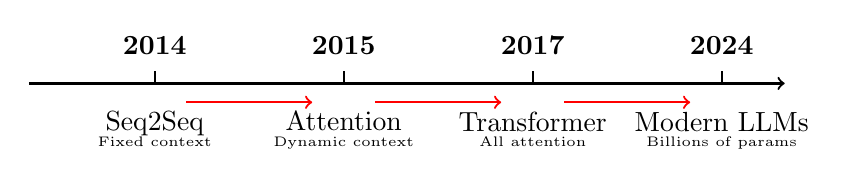
\begin{tikzpicture}[scale=0.8]
        % Timeline
        \draw[thick, ->] (0,0) -- (12,0);
        
        % Key milestones
        \foreach \x/\year/\name/\detail in {
            2/2014/Seq2Seq/Fixed context,
            5/2015/Attention/Dynamic context,
            8/2017/Transformer/All attention,
            11/2024/Modern LLMs/Billions of params
        } {
            \draw[thick] (\x,0) -- (\x,0.2);
            \node[above] at (\x,0.3) {\textbf{\year}};
            \node[below] at (\x,-0.3) {\name};
            \node[below] at (\x,-0.7) {\tiny\detail};
        }
        
        % Impact arrows
        \draw[->, thick, red] (2.5,-0.3) -- (4.5,-0.3);
        \draw[->, thick, red] (5.5,-0.3) -- (7.5,-0.3);
        \draw[->, thick, red] (8.5,-0.3) -- (10.5,-0.3);
    \end{tikzpicture}
    \end{center}
    
    \textbf{Key Innovations:}
    \begin{enumerate}
        \item \textbf{Seq2Seq (2014):} Separate encoding and decoding
        \item \textbf{Attention (2015):} Solve the bottleneck problem
        \item \textbf{Transformer (2017):} Remove RNNs entirely, use only attention
        \item \textbf{GPT/BERT (2018+):} Pre-training on massive data
    \end{enumerate}
    
    \vspace{0.5em}
    \textbf{Key Insight:} Everything you learned today is the foundation of modern LLMs!\\
    \textit{ChatGPT, Claude, and Gemini all build on these seq2seq concepts.}
\end{frame}

% Summary slide
\begin{frame}[t]{Week 4 Summary: Key Takeaways}
    \begin{columns}[T]
        \column{0.5\textwidth}
        \textbf{Problems Solved:}
        \begin{enumerate}
            \item Variable-length I/O
            \item Information bottleneck
            \item Long-range dependencies
            \item Translation alignment
        \end{enumerate}
        
        \vspace{0.5em}
        \textbf{Key Concepts:}
        \begin{itemize}
            \item Encoder-Decoder separation
            \item Context vectors
            \item Teacher forcing
            \item Attention mechanism
            \item Beam search
        \end{itemize}
        
        \column{0.5\textwidth}
        \textbf{You Can Now:}
        \begin{itemize}
            \item Build a seq2seq model
            \item Implement attention
            \item Diagnose bottleneck issues
            \item Choose attention types
            \item Evaluate with BLEU
        \end{itemize}
        
        \vspace{0.5em}
        \textbf{Next Week: Transformers}
        \begin{itemize}
            \item ``Attention is All You Need''
            \item Self-attention
            \item Multi-head attention
            \item Positional encoding
        \end{itemize}
    \end{columns}
    
    \vspace{0.5em}
    \vspace{0.5em}
    \textbf{Quick Review:} Can you explain why we need TWO networks for translation?\\
    \textit{Answer: Because input length $\neq$ output length!}
\end{frame}

\end{document}